\documentclass{scrartcl}

\usepackage[ngerman]{babel}
\usepackage[utf8]{inputenc}
\usepackage[T1]{fontenc}
\usepackage[hidelinks]{hyperref}
\usepackage{graphicx}

\begin{document}
	\title{CodeCamp: Context Awareness, Entwicklung einer Android-App}
	\author{Adrian Kunz, Jan Bingemann, Johann Feser, Michael Prasil, Sven Starcke}
	\date{Kassel, den \today}

	\maketitle
	\vspace*{10ex}
	\begin{figure}[!h]
		\centering
		
\includegraphics{./figures/title.png}
	\end{figure}

	\newpage

	\tableofcontents
	\newpage

	\section{Einleitung}\label{sec:einleitung}
	\paragraph*{Ziele}
	Ziel des Projektes war es, im Rahmen der Veranstaltung \glqq Code Camp 1: Context Awareness\grqq{} eine Android-basierte Anwendung zur Verwaltung und Aufzeichnung der Einkäufe, welche in der ComTec-Küche getätigt werden, zu erstellen.

	\paragraph*{Funktionsweise}
	Auf Basis einer Datenbank können Gegenstände angelegt, gekauft und gelöscht werden.
	Dazu benötigte Nutzer werden ebenfalls in der Datenbank gespeichert.
	Der Zugriff auf diese erfolgt über eine REST-API, welche alle notwendigen Operationen bereitstellt.

	\paragraph*{Überblick}
	Nutzer erhalten bei der Registrierung ein Token, welches für den Zugriff über die REST-API benötigt wird.
	Dieses wird in der Anwendung zwischengespeichert, sodass ein Nutzer mit gültigem Token automatisch angemeldet wird, wenn die Anwendung startet. \\
	Der Fokus der Anwendung liegt auf dem Kauf von Gegenständen.
	Dies ist auf zwei Arten möglich:

	\begin{enumerate}
		\item regulär in der App: Über eine Liste der verfügbaren Gegenstände können solche per Klick zum Warenkorb hinzugefügt werden.

		\item über einen eingebetteten Barcode-Scanner können Gegenstände, deren Barcode bereits in der Datenbank registriert ist dem Warenkorb hinzugefügt werden.
	\end{enumerate}

	Es ist dem Nutzer zudem möglich eine Statistik zur Kaufhäufigkeit der registrierten Gegenstände einzusehen. \\
	Zwecks Verwaltung ist es als Administrator ausgezeichneten Nutzern möglich neue Gegenstände wahlweise mit automatisch generierter ID oder dem Barcode-Scanner anzulegen.

	% REVIEW: Update, wenn neue Sections hinzugefügt werden
	\paragraph*{Inhalt}
	In Abschnitt ~\ref{sec:features} werden die von der App bereitgestellten Features vorgestellt.
	Abschnitt ~\ref{sec:architecture} erklärt die Anwendungsstruktur aus technischer Sicht, jeweils für Datenmodell (Abschnitt ~\ref{subsec:datamodel}), die Oberflächen-Architektur (Abschnitt ~\ref{subsec:frontend}) und die zugrunde liegende Grundstruktur inklusive Netzwerkverkehr (Abschnitt ~\ref{subsec:backend}).


	% REVIEW: neue Features einfügen und ausreichend erklären. Bilder und Referenzen.
	\section{Anwendung}\label{sec:features}
	\paragraph*{Start}
	Beim Öffnen der Anwendung erscheint eine Login-Maske, sofern sich in den Shared-Preferences des Android-Geräts nicht bereits ein gültiges User-Token und eine passende User-Id befinden.
	Sind die Daten vorhanden, wird der Nutzer anhand dieser eingeloggt.
	Falls keine Anmeldedaten vorhanden sind, wird ein neuer Nutzer auf Basis der in der Oberfläche eingegebenen Anmeldedaten (Name, E-Mail, Adminflag, siehe Abbildung ~\ref{loginscreen}) erstellt.
	Das User-Token wird für die weitere Verwendung in den Shared-Preferences zwischengespeichert.

	% Bild vom Login-Screen mit Erklärung
	\begin{figure}[!h]
		\centering
		
\includegraphics[scale=0.5]{./figures/placeholder.png}
		\caption{Login-Screen}
		\label{loginscreen}
	\end{figure}

	\paragraph*{Haupt-Screen}
	Nach erfolgreicher Anmeldung erfolgt eine Weiterleitung auf den Main-Screen.
	Dieser zeigt eine Liste der kaufbaren Gegenstände (siehe Abbildung ~\ref{mainscreen}).

	% Bild vom Main-Screen mit Item-Liste, evtl. Erklärungen anpassen
	\begin{figure}[!h]
		\centering
		
\includegraphics[scale=0.5]{./figures/placeholder.png}
		\caption{Haupt-Screen}
		\label{mainscreen}
	\end{figure}

	Ein Eintrag in dieser Liste enthält folgende Komponenten:

	\begin{itemize}
		\item Den Namen des ausgewählten Gegenstands

		\item Den Preis für einen Gegenstande des ausgewählten Typs

		\item Die ausgewählte Anzahl der Gegenstände des ausgewählten Typs, welche man kaufen möchte.
		Sie erhöht sich mit jedem Klick auf den Eintrag.
		Wischt man hingegen von rechts nach links über den Eintrag, so wird die ausgewählte Anzahl auf 0 gesetzt.
		Die Anzahl wird nur angezeigt, wenn sie größer als 0 ist.

		\item Der Gesamtpreis für den Gegenstandstyp.
		Hierbei handelt es sich um den Kumulierten Preis (ausgewählte Anzahl $\cdot$ Preis) des Gegenstands.
		Dieser wird nur angezeigt, wenn mehr als ein Gegenstand des ausgewählten Typs verlangt wird.

		\item verfügbare Anzahl: Zeigt an, wie viele Gegenstände des ausgewählten Typs gekauft werden können.
		Sie kann aufgrund des Design der REST-API negativ werden.
	\end{itemize}

	Die Liste ist nach der Art der Gegenstände sortiert (Beispiel: Wasser, Saft, \ldots).

	\paragraph*{Gegenstände hinzufügen}
	Ist der aktuelle Nutzer als Administrator ausgezeichnet, kann er mit dem +-Knopf im oberen Banner des Main-Screen neue Gegenstände hinzufügen.
	Dazu müssen folgende Daten eingegeben werden:

	\begin{itemize}
		\item Der Name des zu erstellenden Gegenstands.

		\item Der Preis des zu erstellenden Gegenstands.

		\item Die Menge, in der der Gegenstand verfügbar ist.

		\item Die Art des Gegenstands.
		Hier wird aus einem Drop-Down-Menu eine Art ausgewählt.
	\end{itemize}

	Das Hinzufügen eines Gegenstandes benötigt eine eindeutige ID. Diese wird automatisch generiert und am oberen Bildschirmrand angezeigt (siehe Abbildung ~\ref{createItem}).

	% Bild vom create-Item-Screen, evtl. Erklärungen anpassen
	\begin{figure}[!h]
		\centering
		
\includegraphics[scale=0.5]{./figures/placeholder.png}
		\caption{Erzeugung eines Gegenstandes}
		\label{createItem}
	\end{figure}

	\paragraph*{Gegenstände kaufen}
	Wenn alle gewünschten Gegenstände ausgewählt sind, wird durch einen Klick auf den Einkaufswagen-Button der Warenkorb-Screen geöffnet.
	Hierbei handelt es sich um eine Darstellung nur der ausgewählten Gegenstände mit der bereits bekannten Eintragsstruktur.
	Auch hier können durch einen Klick auf die Einträge Gegenstände hinzugefügt und durch Wischen über einen Eintrag alle Gegenstände dieses Typs entfernt werden.
	Durch einen Klick Löschen-Button kann der komplette Einkauf gelöscht werden.
	Durch einen Klick auf den Submit-Button (Haken) erscheint ein Modal-Fenster (siehe Abbildung ~\ref{shoppingCartCheck}) mit einer Abfrage, ob der Kauf durchgeführt werden soll.
	Hier wird nochmals der Gesamtpreis des Einkaufs angezeigt.
	Beim Klick auf \glqq yes\grqq{} wird der Kauf getätigt und man wird auf den Main-Screen weitergeleitet.
	Durch ein Pop-Up am unteren Bildschrimrand wird gezeigt, dass der Kauf erfolgreich war (siehe Abbildung ~\ref{purchaseSuccess}).

	% Bild des Bestätigungs-Modal, nachdem Haken im Shopping-Cart gecklickt
	\begin{figure}[!h]
		\centering
		
\includegraphics[scale=0.5]{./figures/placeholder.png}
		\caption{Letzte Bestätigung vor Kauf}
		\label{shoppingCartCheck}
	\end{figure}

	% optional: Bild von Benachrichtigung nachdem Kauf erolgreich
	\begin{figure}[!h]
		\centering
		
\includegraphics[scale=0.5]{./figures/placeholder.png}
		\caption{Pop-Up nach erfolgreichem Einkauf}
		\label{purchaseSuccess}
	\end{figure}

	\paragraph*{Verwaltung}
	Mittels des Kontext-Menu-Button in der oberen, rechten Bildschirmecke kann ein Kontext-Menu aufgerufen werden, welches folgende Funktionalität bietet:

	\begin{itemize}
		\item Anzeigen des Nutzernamen im oberen Banner, falls der Nutzer ein Administrator ist, wird dies hinter dem Namen angezeigt.

		\item Link zum Main-Screen: Bei einem Klick erfolgt eine Weiterleitung auf den Main-Screen.

		\item Liste getätigter Einkäufe: Bei einem Klick auf diesen Eintrag erfolgt eine Weiterleitung auf einen Screen, in welchem alle vergangenen Einkäufe nach Datum und Zeit sortiert aufgelistet werden (siehe Abbildung ~\ref{purchases}).

		\item Clear UserData: Bei einem Klick auf diesen Eintrag werden die in den Shared-Preferences gespeicherten Anmeldedaten gelöscht.
		Es erfolgt eine Weiterleitung auf den Login-Screen.
		Eine erneute Anmeldung ist aufgrund des Design der REST-API nicht möglich, ein neuer Nutzer kann jedoch angelegt werden.
	\end{itemize}

	% Bild des Purchases-Screen, evtl. Erklärung anpassen
	\begin{figure}[!h]
		\centering
		
\includegraphics[scale=0.5]{./figures/placeholder.png}
		\caption{Liste getätigter Einkäufe}
		\label{purchases}
	\end{figure}

	\paragraph*{Barcode-Scanner}
	Durch einen Klick auf das Kamera-Icon in der oberen, rechten Ecke des Main-Screen (siehe Abbildung ~\ref{mainscreen}) öffnet sich die Kamera des Gerätes mit einem eingebauten Barcode-Scanner.
	Hiermit kann der Nutzer Barcodes einscannen und Gegenstände anlegen, falls die ID des Barcode nicht in der Datenbank vorhanden ist und der Nutzer ein Administrator ist.
	Alternativ kann der Nutzer den Gegenstand kaufen, falls dieser bereits in der Datenbank registriert ist.

	\section{Architektur}\label{sec:architecture}
	\subsection{Datenmodell}\label{subsec:datamodel}
	\paragraph*{}
	Das Datenmodell umfasst drei Klassen: \texttt{Item}, \texttt{User}, \texttt{Purchase}.
	Die Klassen sind passend zur bereitgestellten Datenbank implementiert und haben die in Abbildung ~\ref{datamodel} gezeigte Struktur.

	\begin{figure}[!h]
		\centering
		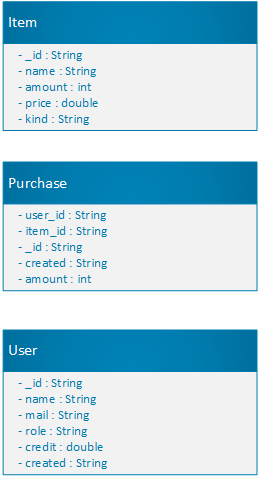
\includegraphics[scale=0.5]{./figures/datamodel.png}
		\caption{Datenmodell}
		\label{datamodel}
	\end{figure}

	\subsection{Frontend-Architektur}\label{subsec:frontend}
	% generelle Architektur (Klassen, verwendete Patterns, Fragments, Activities) und deren grobe Erklärung

	\subsection{Backend-Architektur}\label{subsec:backend}
	\paragraph*{}
	Die Backend-Architektur besteht aus drei Ebenen (siehe Abbildung ~\ref{backendArchitecture}).

	\paragraph*{Base-Layer}
	Die unterste Ebene bildet die Klasse \texttt{OkHttpConnection}, welche über das Interface \texttt{HttpConnection} implementiert ist.
	Die Klasse ist verantwortlich für den primitiven Netzwerkverkehr per HTTP mit beliebigen Inhalten.
	Es werden die HTTP-Methoden \texttt{GET}, \texttt{POST}, \texttt{PUT} und \texttt{DELETE} implementiert.
	Bei fehlerhaften Anfragen (HTTP-Code $\neq$ 2xx), sowie bei fehlerhaften URLs wird eine Exception geworfen.

	\paragraph*{Abstraction-Layer}
	Auf der zweiten Ebene befinden sich die Klassen \texttt{KitchenConnection}, \texttt{LocalDataStore} und \texttt{JsonTranslator}.

	\begin{itemize}
		\item  \texttt{KitchenConnection} ist verantwortlich für die spezialisierte Kommunikation mit der bereitgestellten REST-API. Die Klasse enthält Attribute für die Basis-URL des REST-Servers, sowie für Schlüssel zur Erzeugung von Nutzern.
		Alle Funktionen der REST-API werden hier implementiert, indem jede Methode der Klasse einen Pfad der REST-API abdeckt.
		Die Funktionsnamen entsprechen der Spezifikation der REST-API\@.

		\item \texttt{LocalDataStore} ist verantwortlich für das Zwischenspeichern der User, Items und Purchases.
		Dies ermöglicht schnelleren Zugriff auf die jeweiligen Objekte.

		\item \texttt{JsonTranslator} ist verantwortlich für die bidirektionale Umwandlung zwischen Objekten des Datenmodells und JSON-Strings.
		Die verwendete Bibliothek für die Umwandlung ist Google's \texttt{GSON}.
	\end{itemize}

	\paragraph*{Access-Layer}
	Die Dritte Ebene beinhaltet nur die Klasse \texttt{KitchenManager}.
	Sie ist der Einstiegspunkt des Backend und stellt so alle Operationen zur Verfügung, welche die Oberfläche benötigt. \texttt{KitchenManager} bildet eine vollständige Abstraktion der REST-API, über die Klasse \texttt{KitchenConnection}, welche bereits die Adressen und benötigten Header der API-Aufrufe abstrahierte.

	\begin{figure}[!h]
		\centering
		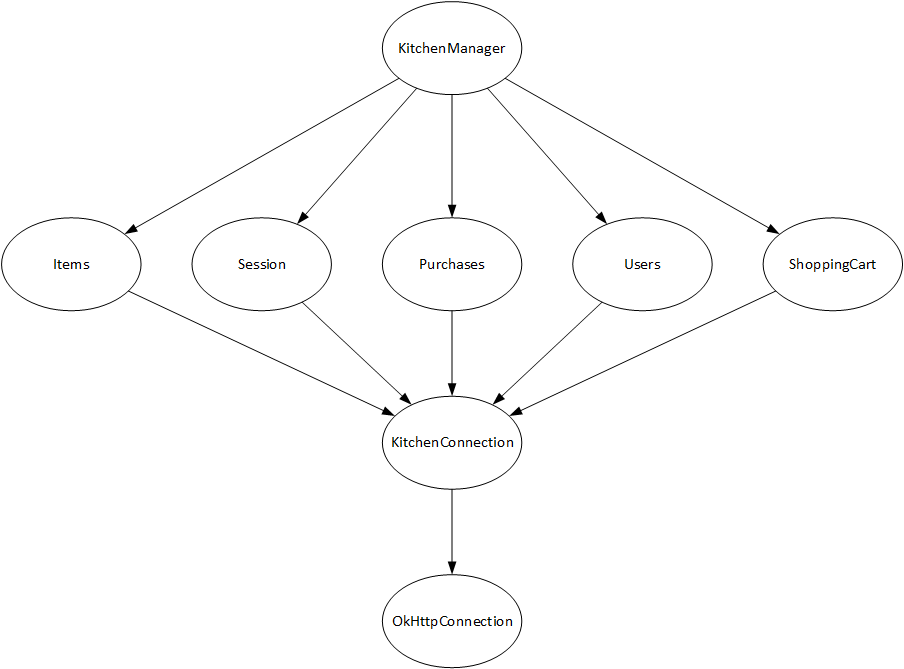
\includegraphics[scale=0.5]{./figures/classStructure.png}
		\caption{Backend Architektur}
		\label{backendArchitecture}
	\end{figure}

	\paragraph*{Tests}
	Alle Backend-Klassen sind durch Unit-, Integrations- und Akzeptanz-Tests ausreichend getestet.

	\section{Anhang: Bibliotheken}\label{sec:bib}
	% alle Benutzten Bibliotheken aufführen

\end{document}
